\documentclass[aspectratio=169, 10pt]{beamer}

% --- Theme and Visual Setup ---
\usetheme{Madrid}
\usecolortheme{whale}
\setbeamertemplate{navigation symbols}{}
\setbeamertemplate{headline}{}

% --- Color Definitions ---
\definecolor{ulbblue}{RGB}{0, 51, 102}
\definecolor{ulbgold}{RGB}{204, 153, 0}
\definecolor{darkred}{RGB}{180, 20, 20}
\definecolor{lightgrey}{RGB}{245, 246, 248}

\setbeamercolor{palette primary}{bg=ulbblue,fg=white}
\setbeamercolor{palette secondary}{bg=ulbblue!80!black,fg=white}
\setbeamercolor{palette tertiary}{bg=ulbblue!60!black,fg=white}
\setbeamercolor{structure}{fg=ulbblue}
\setbeamercolor{frametitle}{bg=ulbblue,fg=white}
\setbeamercolor{block title}{bg=ulbblue,fg=white}
\setbeamercolor{block body}{bg=lightgrey,fg=black}
\setbeamercolor{block title alerted}{bg=darkred,fg=white}
\setbeamercolor{block body alerted}{bg=lightgrey,fg=black}

% --- Packages ---
\usepackage[utf8]{inputenc}
\usepackage[T1]{fontenc}
\usepackage{amsmath, amssymb, amsfonts}
\usepackage{physics}
\usepackage{siunitx}
\usepackage{booktabs}
\usepackage{tikz}
\usetikzlibrary{arrows.meta, calc, positioning, shapes.geometric}

\usepackage{caption}
\usepackage{mathtools}  
\mathtoolsset{showonlyrefs} % TO REMOVE QUEATION NUMBERING IF NOT CITED/REFERENCED

\newcommand{\km}{km} % FIX for siunitx ?
\newcommand{\kilo}{k}
\newcommand{\meter}{m}
\newcommand{\metre}{m}

% --- Presentation Metadata ---
\title[Ionospheric OTH Radar Detection]{Ionospheric Reflections and Over-The-Horizon Naval Radar}
\subtitle{ELEC-H415 - Chapter 5}
\author[Lucas Placentino]{Lucas Placentino}
\institute[EPB-ULB]{
    École polytechnique de Bruxelles \\
    Université libre de Bruxelles
}
\date{2026}


\begin{document}

% =============================================================================
% SLIDE 1: Title Slide
% =============================================================================
\begin{frame}
    \titlepage
\end{frame}

% =============================================================================
% SLIDE 2: Operational Context & Physical Problem
% =============================================================================

\begin{frame}{Context: Over-The-Horizon (OTH) Threat Detection}
    \begin{columns}[T]
        \begin{column}{0.52\textwidth}
            \begin{block}{The Line-of-Sight Microwave Horizon}
                Standard naval microwave radars ($\sim \SI{3}{\giga\hertz} - \SI{10}{\giga\hertz}$) are limited by Earth curvature:
                \begin{equation}
                    d_{\text{LOS}} \approx \sqrt{2 k_e R_e}\left(\sqrt{h_{\text{mast}}} + \sqrt{h_{\text{target}}}\right) \approx \mathbf{30 - 50\,\si{\km}}
                \end{equation}
                A warship cannot detect threats beyond this optical horizon.
            \end{block}
        \end{column}
        \begin{column}{0.45\textwidth}
            \begin{alertblock}{The Skywave Reflection Radar}
                \textbf{Over-The-Horizon (OTH) Radar} exploits total reflection on the \textbf{ionosphere} in a lower frequency band, achieving detection ranges up to $\mathbf{4000\,\si{\km}}$.
            \end{alertblock}
            \vspace{0.1cm}
            \textbf{Theoretical Goals of this Lesson:}
            \begin{itemize}
                \item Plasma frequency \& electron density profile $n_e(h)$.
                \item Total Internal Reflection condition via Snell's Law.
                \item Prove the Secant Law ($f_{\max} = f_p/\cos\theta_i$).
                \item Analyze the Skip Zone \& Tropospheric Limits.
            \end{itemize}
        \end{column}
    \end{columns}
\end{frame}

% =============================================================================
% SLIDE 3: Lesson Roadmap
% =============================================================================
% \begin{frame}{Lesson Roadmap}
%     \tableofcontents
% \end{frame}

% =============================================================================
% SECTION 1: Plasma Electrodynamics & Permittivity
% =============================================================================
\section{Ionospheric Plasma Physics \& Electron Density Profiles}

\begin{frame}{Ionospheric Plasma \& Electron Density Profile $n_e(h)$}
    \begin{columns}[c]
        \begin{column}{0.52\textwidth}
            \begin{block}{Plasma Relative Permittivity}
                The ionosphere acts as a plasma layer with relative permittivity:
                \begin{equation}
                    \mathbf{\varepsilon_r(\omega) = 1 - \frac{\omega_p^2}{\omega^2} < 1} \quad \text{with} \quad \omega_p = \sqrt{\frac{n_e q_e^2}{m_e \varepsilon_0}}
                \end{equation}
            \end{block}
            \begin{itemize}
                \item $n_e(h)$: Free electron volume density $[\si{\m^{-3}}]$.
                \item Its variation is caused by solar activity.
                % \item \textbf{Day}: Stratification into $D, E, F_1, F_2$ layers.
                % \item \textbf{Night}: Lower layers vanish; $F_1, F_2$ merge into a single, higher $F$ layer ($h \sim \SI{450}{\km}$).
            \end{itemize}
        \end{column}
        \begin{column}{0.45\textwidth}
            \centering
            % --- Figure 5.9: Day vs Night Ionosphere Profile ---
            \begin{figure}
                \centering
                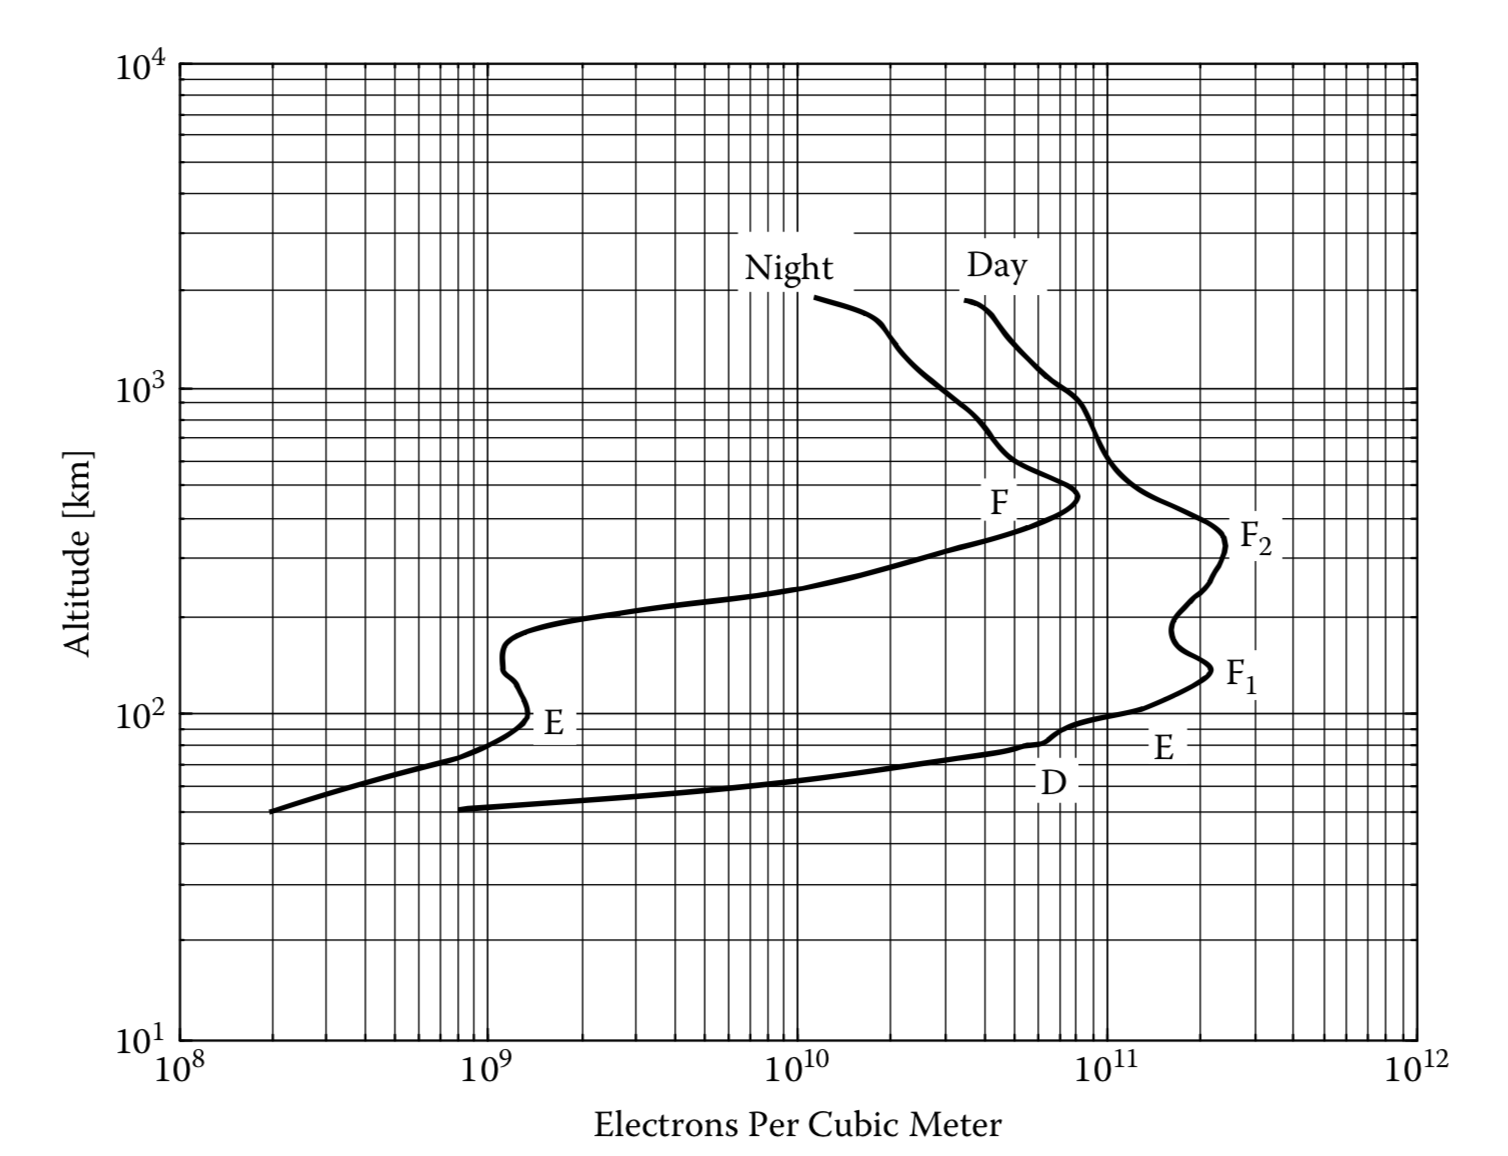
\includegraphics[width=1\linewidth]{electrons-ionosphere.png}
                \caption{\footnotesize Electron density $n_e$ in the ionosphere (Source : V.L. Granatstein, \textit{Physical principles of wireless communications}, Auerbach, 2008)}
            \end{figure}
            % \begin{tikzpicture}[scale=0.82]
            %     % Grid / Axes
            %     \draw[thick, ->] (0,0) -- (4.8,0) node[right] {\footnotesize $n_e\,[\si{\m^{-3}}]$};
            %     \draw[thick, ->] (0,0) -- (0,3.8) node[above] {\footnotesize Altitude $h\,[\si{\km}]$};
                
            %     % Ticks X (log scale)
            %     \node at (0.8,-0.25) {\tiny $10^9$};
            %     \node at (2.0,-0.25) {\tiny $10^{10}$};
            %     \node at (3.2,-0.25) {\tiny $10^{11}$};
            %     \node at (4.4,-0.25) {\tiny $10^{12}$};
                
            %     % Ticks Y
            %     \node at (-0.35,0.6) {\tiny $60$};
            %     \node at (-0.35,1.2) {\tiny $120$};
            %     \node at (-0.35,2.1) {\tiny $300$};
            %     \node at (-0.35,3.2) {\tiny $600$};
                
            %     \draw[dotted, lightgray] (0,0.6) -- (4.5,0.6);
            %     \draw[dotted, lightgray] (0,1.2) -- (4.5,1.2);
            %     \draw[dotted, lightgray] (0,2.1) -- (4.5,2.1);
            %     \draw[dotted, lightgray] (0,3.2) -- (4.5,3.2);

            %     % Day Curve (Red)
            %     \draw[thick, darkred, smooth] plot coordinates {
            %         (0.3,0.3) (0.9,0.6) (2.2,1.2) (3.2,1.8) (3.8,2.2) (3.5,3.0) (2.3,3.6)
            %     };
            %     \node[darkred, right] at (3.4,2.2) {\footnotesize \textbf{Day}};
            %     \node[darkred] at (1.1,0.75) {\tiny $D$};
            %     \node[darkred] at (2.4,1.35) {\tiny $E$};
            %     \node[darkred] at (3.4,1.7) {\tiny $F_1$};
            %     \node[darkred] at (4.0,2.4) {\tiny $F_2$};

            %     % Night Curve (Blue Dashed)
            %     \draw[thick, ulbblue, dashed, smooth] plot coordinates {
            %         (0.4,1.2) (1.2,1.6) (2.8,2.5) (1.8,3.5)
            %     };
            %     \node[ulbblue, left] at (2.8,2.7) {\footnotesize \textbf{Night ($F$)}};
            % \end{tikzpicture}
            % \captionof{figure}{\footnotesize $n_e(h)$ profile (Granatstein / Fig. 5.9)}
        \end{column}
    \end{columns}
\end{frame}

\begin{frame}{Fundamental Plasma Frequency \& Plasma Refractive Index}
\small
    Substituting physical constants into $f_p = \frac{\omega_p}{2\pi}$:
    \begin{itemize}
        \item Elementary charge: $q_e \approx \SI{1.60217663e-19}{\coulomb}$
        \item Electron mass: $m_e \approx \SI{9.1093837e-31}{\kilo\gram}$
        \item Vacuum permittivity: $\varepsilon_0 \approx \SI{8.8541878e-12}{\farad\per\m}$
    \end{itemize}
    \begin{align}
        f_p &= \frac{1}{2\pi} \sqrt{\frac{q_e^2}{m_e \varepsilon_0}} \sqrt{n_e} = \frac{1}{2\pi} \sqrt{\frac{(1.60218\times 10^{-19})^2}{9.10938\times 10^{-31} \times 8.85419\times 10^{-12}}} \sqrt{n_e} \nonumber \\
        &= \frac{1}{2\pi} \sqrt{3.1826 \times 10^3} \sqrt{n_e} = \frac{56.415}{2\pi} \sqrt{n_e} \approx \mathbf{8.9788 \sqrt{n_e}}
    \end{align}
    \begin{equation}
        \implies \mathbf{f_p \approx 8.98 \sqrt{n_e}}\quad [\si{\hertz}] \quad (\text{with } n_e \text{ in } [\si{\m^{-3}}])
    \end{equation}

    \begin{alertblock}{Refractive Index of the Plasma}
        Assuming non-magnetic medium ($\mu = \mu_0$):
        \begin{equation}
            n = \frac{c}{v} = \frac{\sqrt{\varepsilon \mu_0}}{\sqrt{\varepsilon_0\mu_0}} = \sqrt{\varepsilon_r} = \sqrt{1 - \frac{\omega_p^2}{\omega^2}} = \sqrt{1 - \frac{f_p^2}{f^2}} < 1
        \end{equation}
        Because $n < 1$, the ionosphere is an \textbf{optically less dense medium} than the neutral troposphere ($n_{\text{air}} \approx 1$).
    \end{alertblock}
\end{frame}

% =============================================================================
% SECTION 2: Boundary Value Problem & Total Internal Reflection
% =============================================================================
\section{Boundary Value Problem \& Fresnel Total Reflection}

\section{Boundary Value Problem \& Total Internal Reflection}

\begin{frame}{Total Internal Reflection at the Ionospheric Boundary}
    \begin{columns}[c]
        \begin{column}{0.55\textwidth}
            Consider an EM wave incident on the ionospheric layer:
            \begin{itemize}
                \item \textbf{Below the ionosphere}: $\varepsilon_{r1} \approx 1 \implies n_1 \approx 1$
                \item \textbf{In the ionosphere}: $\varepsilon_{r2} = 1 - \frac{\omega_p^2}{\omega^2} < 1 \implies n_2 < n_1$
            \end{itemize}
            We can use \textbf{Snell's Law} at the interface:
            \begin{equation}
                n_2 \sin\theta_2 = n_1 \sin\theta_1 \implies \sin\theta_2 = \frac{n_1}{n_2} \sin\theta_i = \frac{\sin\theta_i}{\sqrt{\varepsilon_r}}
            \end{equation}
            Since $n_2 < n_1$, $\sin\theta_2$ can become **greater than 1**!
            
            \vspace{0.1cm}
            %\textbf{Fresnel Perpendicular Reflection Coefficient:}
            \textbf{Perpendicular Reflection Coefficient:}
            \begin{equation}
                \Gamma_\perp(\theta_i) = \frac{\cos\theta_i - \sqrt{\varepsilon_r - \sin^2\theta_i}}{\cos\theta_i + \sqrt{\varepsilon_r - \sin^2\theta_i}}
            \end{equation}
        \end{column}
        \begin{column}{0.42\textwidth}
            \begin{block}{Critical Angle $\theta_c$}
                Total reflection happens when the transmitted wave angle reaches $\theta_2 = \pi/2$ ($\sin\theta_2 = 1$):
                \begin{equation}
                    \sin\theta_c = \sqrt{\frac{\varepsilon_2}{\varepsilon_1}} = \sqrt{1 - \frac{\omega_p^2}{\omega^2}} = \sqrt{1 - \frac{f_p^2}{f^2}}
                \end{equation}
            \end{block}
            \begin{alertblock}{Condition for Total Reflection}
                Total reflection happens whenever $\theta_i \ge \theta_c$:
                \begin{equation}
                    \mathbf{\sin\theta_i \ge \sqrt{1 - \frac{f_p^2}{f^2}}}
                \end{equation}
            \end{alertblock}
        \end{column}
    \end{columns}
\end{frame}

\begin{frame}{Derivation of the Maximum Usable Frequency}
\small
    From the total reflection condition:
    \begin{equation}
        \sin^2\theta_i \ge 1 - \frac{f_p^2}{f^2}
    \end{equation}
    Rearranging:
    \begin{equation}
        \frac{f_p^2}{f^2} \ge 1 - \sin^2\theta_i = \cos^2\theta_i
    \end{equation}
    Taking the square root (since all frequencies and cosines are non-negative):
    \begin{equation}
        \frac{f_p}{f} \ge \cos\theta_i \iff f \le \frac{f_p}{\cos\theta_i} = f_p \sec\theta_i
    \end{equation}
\vspace{-0.6em}
    \begin{alertblock}{\small The Secant Law for OTH Radar}
        For a given incidence angle $\theta_i$, total reflection occurs for all frequencies up to:
        \begin{equation}
            \mathbf{f_{\max} = \frac{f_{p,\max}}{\cos\theta_i}}
        \end{equation}
        \begin{itemize}
            \item \textbf{Vertical Incidence} ($\theta_i = 0^\circ \implies \cos\theta_i = 1$): $f_{\max} = f_p$.
            \item \textbf{Oblique Naval Incidence} ($\theta_i \to 80^\circ \implies \cos\theta_i \approx 0.17$): $f_{\max} \approx 5.8 \times f_p \approx 20-\SI{30}{\mega\hertz}$.
        \end{itemize}
    \end{alertblock}
\end{frame}

% =============================================================================
% SECTION 3: Spherical Earth Geometry & Radar Hop Footprint
% =============================================================================
\section{Spherical Earth Geometry \& Coverage Footprint}

\begin{frame}{Spherical Earth Geometry for Grazing Single-Hop Detection}
    \begin{columns}[c]
        \begin{column}{0.55\textwidth}
            To maximize detection range, the warship radiates at grazing elevation ($E \approx 0^\circ$, tangent to Earth):

            \vspace{0.15cm}
            \textbf{1. Angle of Incidence $\theta_i$ at Height $h_i$:}
            From the right-angle triangle ($\triangle O T I$):
            \begin{equation}
                \sin\theta_i = \frac{R_e}{R_e + h_i} \quad (R_e = \SI{6375}{\km})
            \end{equation}
            \textbf{2. Angle at Earth Center $\alpha$:}
            \begin{equation}
                \alpha = \frac{\pi}{2} - \theta_i
            \end{equation}
            \textbf{3. Maximal Single-Hop Ground Arc $d_{\max}$:}
            \begin{equation}
                \mathbf{d_{\max} = 2 R_e \alpha = 2 R_e \left(\frac{\pi}{2} - \theta_i\right)}
            \end{equation}
        \end{column}
        \begin{column}{0.42\textwidth}
        \begin{figure}
            \centering
            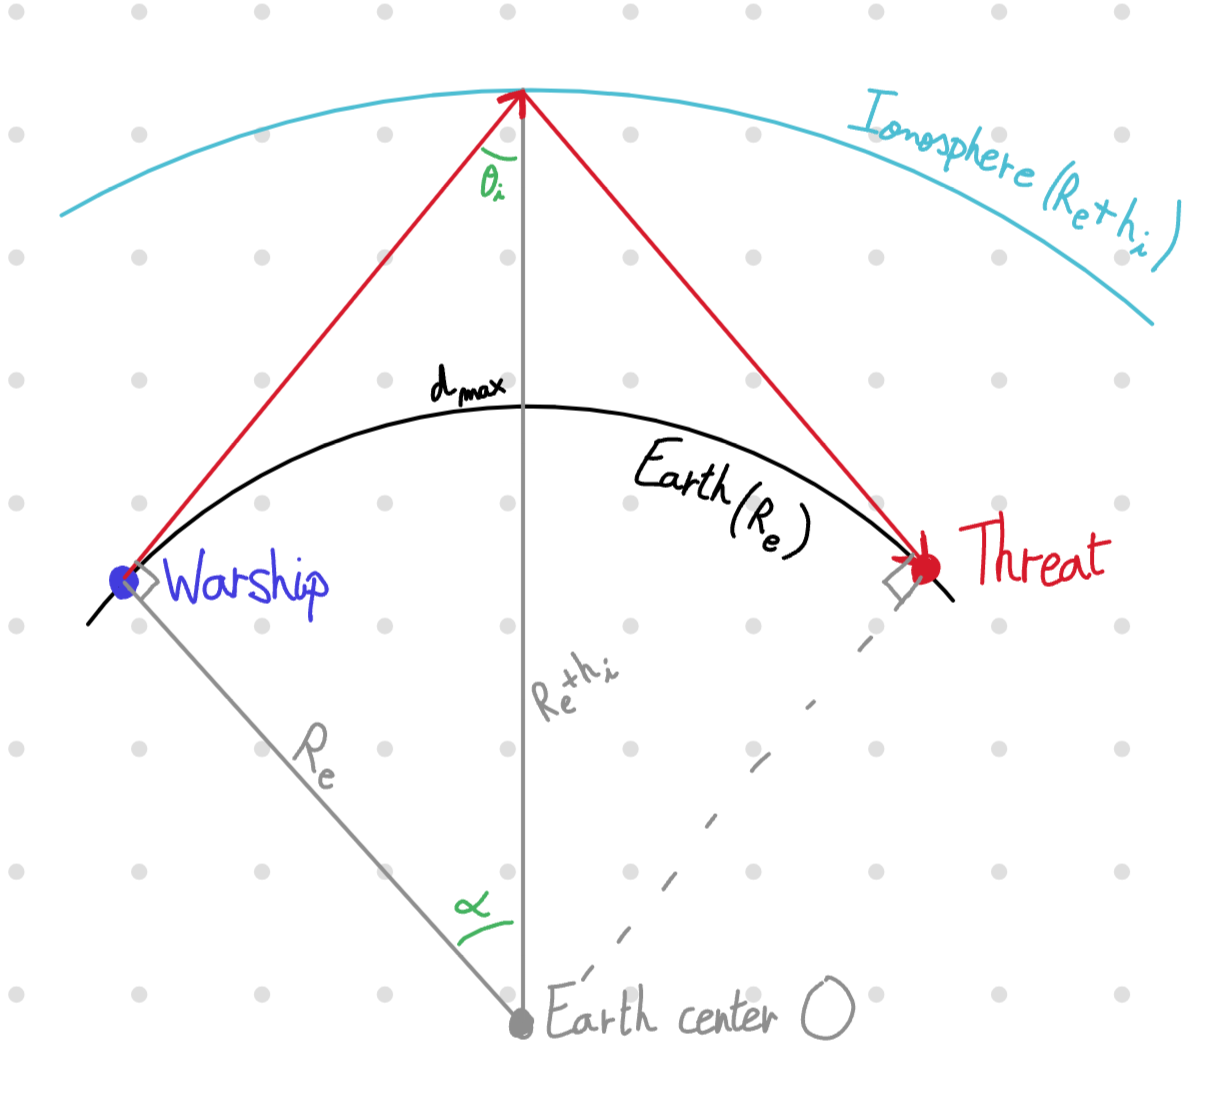
\includegraphics[width=1\linewidth]{earth-and-ionosphere-radar.png}
            % \caption{Enter Caption}
        \end{figure}
            % \begin{tikzpicture}[scale=0.95]
            %     % Earth surface
            %     \draw[thick] (0,1) arc (130:50:3cm);
            %     \node at (4.2,1.0) [below] {\footnotesize Earth ($R_e$)};
            %     % Ionosphere
            %     \draw[thick, dashed, ulbblue] (-0.4,1.9) arc (130:50:3.8cm);
            %     \node at (4.4,2.5) [above, ulbblue] {\footnotesize Layer ($R_e+h_i$)};
            %     % Earth center
            %     \coordinate (O) at (1.9,-1.8);
            %     \filldraw (O) circle (1.5pt) node[below] {\footnotesize Earth Center $O$};
            %     % Vectors
            %     \draw[dashed] (O) -- (0.4,1.3) node[midway, left] {\footnotesize $R_e$};
            %     \draw[dashed] (O) -- (1.9,2.8) node[midway, right] {\footnotesize $R_e+h_i$};
            %     % Ray path
            %     \draw[thick, darkred, ->, >=stealth] (0.4,1.3) node[left, blue] {\footnotesize Warship} -- (1.9,2.8);
            %     \draw[thick, darkred, ->, >=stealth] (1.9,2.8) -- (3.4,1.3) node[right, red] {\footnotesize Target};
            %     \node at (1.9,1.5) {\footnotesize $d_{\max}$};
            % \end{tikzpicture}
        \end{column}
    \end{columns}
\end{frame}

\begin{frame}{Applied Day vs. Night Detection Rnage Comparison}
    \begin{columns}[T]
        \begin{column}{0.48\textwidth}
            %\begin{block}{Daytime Mission ($F_1$ Layer)}
            \begin{block}{Daytime}
                High solar activity:
                \begin{itemize}
                    \item Layer height: $h_i \approx \SI{120}{\km}$
                    \item Peak electron density: $n_{e,\max} \approx \SI{2e11}{\m^{-3}}$
                \end{itemize}
                \textbf{Step-by-Step Derivation:}
                \begin{enumerate}
                    \item $f_{p,\max} = 8.98\sqrt{2\times 10^{11}} = \mathbf{4.02\,\si{\mega\hertz}}$
                    \item $\sin\theta_i = \frac{6375}{6495} = 0.9815 \implies \mathbf{\theta_i = 78.97^\circ}$
                    \item $f_{\max} = \frac{4.02}{\cos(78.97^\circ)} = \frac{4.02}{0.1913} = \mathbf{21.0\,\si{\mega\hertz}}$
                    \item $d_{\max} = 2 \times 6375 \left(\frac{\pi}{2} - 1.3783\right) = \mathbf{2248\,\si{\km}}$
                \end{enumerate}
            \end{block}
        \end{column}
        \begin{column}{0.48\textwidth}
            %\begin{block}{Nighttime Mission ($F$ Layer)}
            \begin{block}{Nighttime}
                Low solar activity:
                \begin{itemize}
                    \item Layer height: $h_i \approx \SI{450}{\km}$
                    \item Peak electron density: $n_{e,\max} \approx \SI{8e10}{\m^{-3}}$
                \end{itemize}
                \textbf{Step-by-Step Derivation:}
                \begin{enumerate}
                    \item $f_{p,\max} = 8.98\sqrt{8\times 10^{10}} = \mathbf{2.54\,\si{\mega\hertz}}$
                    \item $\sin\theta_i = \frac{6375}{6825} = 0.9341 \implies \mathbf{\theta_i = 69.08^\circ}$
                    \item $f_{\max} = \frac{2.54}{\cos(69.08^\circ)} = \frac{2.54}{0.3571} = \mathbf{7.11\,\si{\mega\hertz}}$
                    \item $d_{\max} = 2 \times 6375 \left(\frac{\pi}{2} - 1.2057\right) = \mathbf{4650\,\si{\km}}$
                \end{enumerate}
            \end{block}
        \end{column}
    \end{columns}

    \begin{alertblock}{Time of Day Conclusion}
        Nighttime doubles the single-hop range ($\mathbf{4650\,\si{\km}}$), but the radar frequency must be lowered to $\mathbf{7.1\,\si{\mega\hertz}}$ to prevent the wave from escaping into space.
    \end{alertblock}
\end{frame}

% =============================================================================
% SECTION 4: Elevation Angle Mapping & The Skip Zone
% =============================================================================
\section{Elevation Angle Mapping \& The Skip Zone}

\begin{frame}{Elevation Angle $E$ to Incidence Angle $\theta_i$ Relationship}
    \begin{columns}[c]
        \begin{column}{0.55\textwidth}
            For non-grazing, with elevation angle $E > 0^\circ$:
            
            \vspace{0.1cm}
            In triangle $\triangle O T I$ (Earth center $O$, warship $T$, ionosphere $I$):
            \begin{itemize}
                \item Angle at $T$: $\frac{\pi}{2} + E$
                \item Angle at $I$: $\pi - \theta_i$ (so $\sin(\pi - \theta_i) = \sin\theta_i$)
            \end{itemize}
            By the \textbf{law of sines}:
            \begin{equation}
                \frac{\sin\theta_i}{R_e} = \frac{\sin\left(\frac{\pi}{2} + E\right)}{R_e + h_i} = \frac{\cos E}{R_e + h_i}
            \end{equation}
            \begin{equation}
                \implies \mathbf{\sin\theta_i(E) = \frac{R_e}{R_e + h_i} \cos E}
            \end{equation}
            The angle at earth center is:
            \begin{equation}
                \alpha(E) = \frac{\pi}{2} - E - \theta_i(E)
            \end{equation}
        \end{column}
        \begin{column}{0.42\textwidth}
            \begin{block}{Range vs. Elevation $E$}
                \begin{equation}
                    d(E) = 2 R_e \left(\frac{\pi}{2} - E - \arcsin\left(\frac{R_e\cos E}{R_e + h_i}\right)\right)
                \end{equation}
            \end{block}
            \begin{alertblock}{Physical Interpretation}
                As the radar antenna tilts upward ($E \uparrow$):
                \begin{itemize}
                    \item $\theta_i$ decreases (steeper incidence).
                    \item Ground range $d(E)$ decreases.
                    \item $\cos\theta_i$ increases, requiring higher plasma density to reflect.
                \end{itemize}
            \end{alertblock}
        \end{column}
    \end{columns}
\end{frame}

\begin{frame}{Derivation of the Radar "Skip/Blind Zone"}
% \small
    Suppose the warship operates at fixed frequency $f > f_p$ (e.g. $f = \SI{15}{\mega\hertz}$).
    
    \vspace{0.1cm}
    Total internal reflection requires $\cos\theta_i \le \frac{f_p}{f}$, which imposes a \textbf{minimum incidence angle $\theta_{i,\min}$}:
    \begin{equation}
        \cos\theta_{i,\min} = \frac{f_p}{f} \implies \sin\theta_{i,\min} = \sqrt{1 - \left(\frac{f_p}{f}\right)^2}
    \end{equation}
    Rays launched at steeper angles ($\theta_i < \theta_{i,\min}$) escape to space. The maximum elevation angle that still reflects is:
    \begin{equation}
        \cos E_{\max} = \frac{R_e + h_i}{R_e} \sin\theta_{i,\min} = \frac{R_e + h_i}{R_e}\sqrt{1 - \left(\frac{f_p}{f}\right)^2}
    \end{equation}
\vspace{-0.6em}
    \begin{alertblock}{\small Skip/Blind Distance ($d_{\text{skip}}$)}
        \small
        The minimum distance at which skywave radar returns to Earth is the \textbf{Skip Distance}:
        % \vspace{-0.6em}
        \begin{equation}
            \mathbf{d_{\text{skip}} = 2 R_e \left(\frac{\pi}{2} - E_{\max} - \theta_{i,\min}\right)}
        % \vspace{-0.4em}
        \end{equation}
    \end{alertblock}
\end{frame}

\begin{frame}{Example of Skip Distance}
    \textbf{Skip distance}: $\mathbf{d_{\text{skip}} = 2 R_e \left(\frac{\pi}{2} - E_{\max} - \theta_{i,\min}\right)}$\\

    \begin{figure}
        \centering
        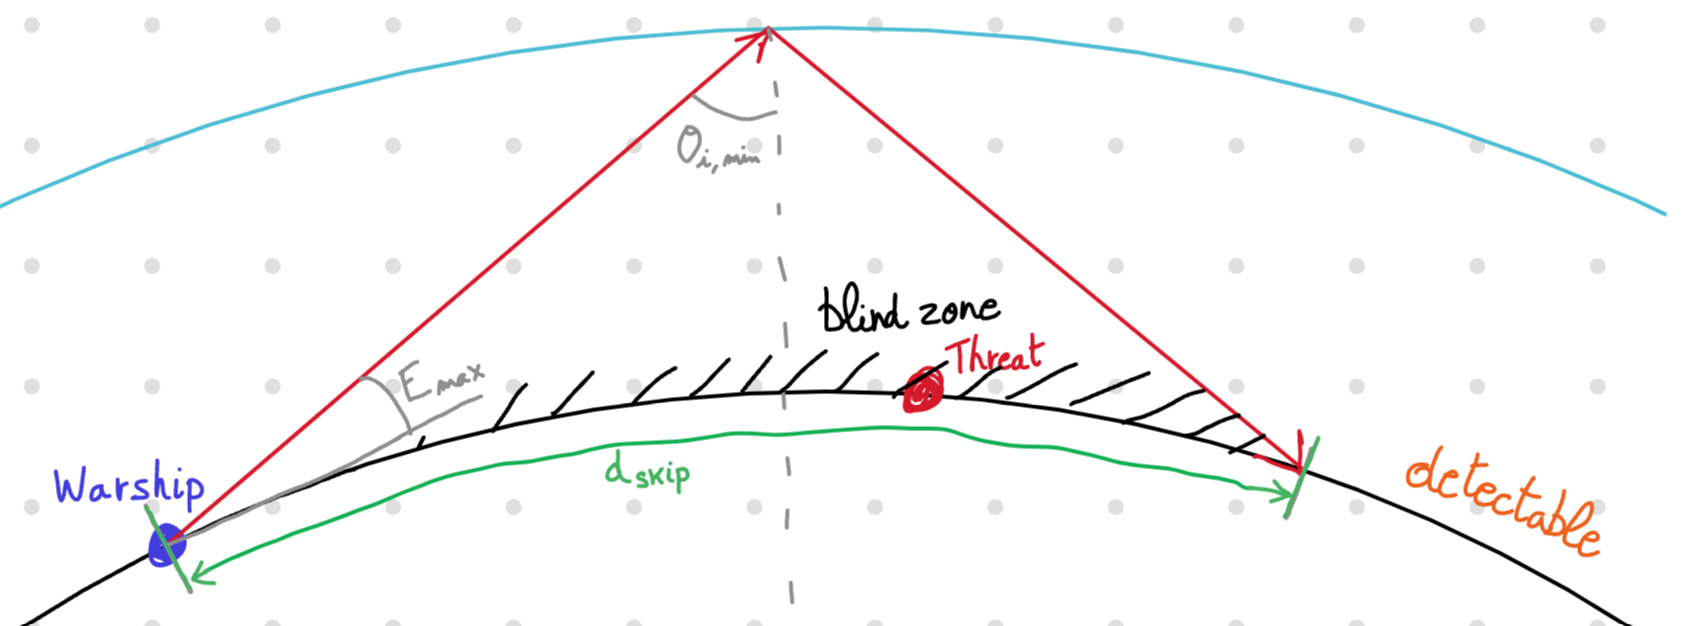
\includegraphics[width=0.75\linewidth]{blind-zone.png}
    \end{figure}
    
    \textbf{Example}, daytime ($f = \SI{15}{\mega\hertz}, f_p = \SI{4.02}{\mega\hertz}, h_i = \SI{120}{\km}$):
        \begin{itemize}
            \item $\theta_{i,\min} = \arccos(4.02/15) = 74.46^\circ = \SI{1.300}{\radian}$
            \item $\cos E_{\max} = \frac{6495}{6375}\sqrt{1 - (4.02/15)^2} = 1.0188 \times 0.9635 = 0.9816 \implies E_{\max} = 11.0^\circ = \SI{0.192}{\radian}$
            \item $d_{\text{skip}} = 2 \times 6375 \times \left(\frac{\pi}{2} - 0.192 - 1.300\right) = 2 \times 6375 \times 0.0788 \approx \mathbf{1005\,\si{\km}}$
        \end{itemize}
\end{frame}

% =============================================================================
% SECTION 5: Bridging the Skip Zone (LOS & Tropospheric Refraction)
% =============================================================================
\section{Can Line-of-Sight or Tropospheric Refraction Bridge the Skip Zone?}

\begin{frame}{Line-of-Sight vs. Tropospheric Ray Bending in the Blind Zone}
\small
    \begin{block}{Fixing the Problem}
        Can we detect a threat located inside the \textbf{Blind Zone} ($d < d_{\text{skip}} \approx \SI{1000}{\km}$) using direct Line-of-Sight (\textbf{LOS}) or \textbf{Tropospheric Ray Bending} ($k_e \approx 4/3$)?
    \end{block}
    \vspace{-0.4em}
    \begin{columns}[T]
        \begin{column}{0.48\textwidth}
            \textbf{1. Pure Geometric Horizon ($k_e = 1$):}
            No atmospheric refraction ($R_{\text{eff}} = R_e = \SI{6375}{\km}$):
            \begin{equation}
                d_{\text{geom}} \approx \sqrt{2 R_e h_{\text{mast}}} + \sqrt{2 R_e h_{\text{target}}}
            \end{equation}
            With $\sqrt{2 R_e} \approx \SI{3.571}{\km\per\sqrt{\m}}$:
            \begin{itemize}
                \item Warship mast: $h_{\text{mast}} = \SI{25}{\m}$
                \item Threat: $h_{\text{target}} = \SI{10}{\m}$
            \end{itemize}
            \begin{align}
                d_{\text{geom}} &= 3.571 \times \left(\sqrt{25} + \sqrt{10}\right) \nonumber \\
                &= 3.571 \times (5 + 3.162) = \mathbf{29.15\,\si{\km}}
            \end{align}
        \end{column}
        \begin{column}{0.48\textwidth}
            \textbf{2. With Tropospheric Bending ($k_e = 4/3$):}
            Downward ray curvature ($R_{\text{eff}} = \SI{8500}{\km}$):
            \begin{equation}
                d_{\text{tropo}} \approx \sqrt{2 k_e R_e}\left(\sqrt{h_{\text{mast}}} + \sqrt{h_{\text{target}}}\right)
            \end{equation}
            With $\sqrt{2 k_e R_e} \approx \SI{4.123}{\km\per\sqrt{\m}}$:
            \begin{align}
                d_{\text{tropo}} &= 4.123 \times \left(\sqrt{25} + \sqrt{10}\right) \nonumber \\
                &= 4.123 \times 8.162 = \mathbf{33.65\,\si{\km}}
            \end{align}
            \vspace{-2em}
            \begin{alertblock}{Tropospheric Effect Advantage}
                Here ray bending extends the threat horizon by only:
                \vspace{-1em}
                \begin{equation}
                    \Delta d = 33.65 - 29.15 = \mathbf{+4.5\,\si{\km}}
                \end{equation}
            \end{alertblock}
        \end{column}
    \end{columns}
\end{frame}

\begin{frame}{Target Altitude Impact \& Radar Coverage Analysis}
    What if the incoming threat is a high-altitude aircraft ($h_{\text{target}} = \SI{10\,000}{\m} = \SI{10}{\km}$)?
    \begin{align}
        d_{\text{geom}} &= 3.571 \times \left(\sqrt{25} + \sqrt{10\,000}\right) = 3.571 \times (5 + 100) = \mathbf{375.0\,\si{\km}} \\
        d_{\text{tropo}} &= 4.123 \times \left(\sqrt{25} + \sqrt{10\,000}\right) = 4.123 \times (5 + 100) = \mathbf{432.9\,\si{\km}}
    \end{align}

    \begin{table}[h]
        \centering
        \small
        \begin{tabular}{lcccc}
            \toprule
            \textbf{Target Threat} & \textbf{Geometric Horizon} & \textbf{Tropospheric Bending} & & \textbf{Skywave Min Distance} \\ \midrule
            \textbf{Sea-level} ($h=\SI{10}{\m}$) & $\SI{29.2}{\km}$ & $\mathbf{33.7\,\si{\km}}$ & $\mathcolor{red}{\longleftrightarrow}$ & $\SI{1005}{\km}$ \\
            \textbf{Low-alt} ($h=\SI{500}{\m}$) & $\SI{97.7}{\km}$ & $\SI{112.8}{\km}$ & $\mathcolor{orange}{\longleftrightarrow}$ & $\SI{1005}{\km}$ \\
            \textbf{High-alt} ($h=\SI{10}{\km}$) & $\SI{375.0}{\km}$ & $\SI{432.9}{\km}$ & $\mathcolor{yellow}{\longleftrightarrow}$ & $\SI{1005}{\km}$ \\ \bottomrule
        \end{tabular}
    \end{table}

    \begin{alertblock}{Conclusion}
        \begin{itemize}
            \item Neither pure LOS nor standard tropospheric ray-bending can bridge the entire blind gap of Skywave radars.
            \item Need to deploy other technologies to cover this skip zone.
        \end{itemize}
    \end{alertblock}
\end{frame}

% =============================================================================
% SECTION 6: Geometric Slant Path & Power Sizing
% =============================================================================
% \section{Geometric Slant Path \& Skywave Power Budget}

% \begin{frame}{Slant Path Length \& Free-Space Spreading Loss}
% \small
%     \begin{columns}[c]
%         \begin{column}{0.55\textwidth}
%             For an OTH single hop covering ground distance $d$, the ray travels along two triangular slant paths of length $s/2$:
            
%             \vspace{0.1cm}
%             Applying the **Law of Cosines** on $\triangle O T I$ with central half-angle $\alpha = \frac{d}{2 R_e}$:
%             \begin{equation}
%                 \left(\frac{s}{2}\right)^2 = R_e^2 + (R_e + h_i)^2 - 2 R_e (R_e + h_i)\cos\left(\frac{d}{2 R_e}\right)
%             \end{equation}
%             \begin{equation}
%                 \implies s(d) = 2 \sqrt{R_e^2 + (R_e + h_i)^2 - 2 R_e (R_e + h_i)\cos\left(\frac{d}{2 R_e}\right)}
%             \end{equation}
%             Under our proven condition of total reflection ($|\Gamma| = 1$), the only geometric attenuation along the skywave path is **free-space spreading**:
%             \begin{equation}
%                 L_{\text{FS}} = \left(\frac{4\pi s}{\lambda}\right)^2 = \left(\frac{4\pi s f}{c}\right)^2
%             \end{equation}
%         \end{column}
%         \begin{column}{0.42\textwidth}
%             \begin{block}{Numerical Slant Sizing ($d = \SI{2000}{\km}$)}
%                 \begin{itemize}
%                     \item $h_i = \SI{120}{\km}$, $R_e = \SI{6375}{\km}$
%                     \item $\alpha = \frac{1000}{6375} = \SI{0.15686}{rad} \approx 8.987^\circ$
%                 \end{itemize}
%                 \begin{align}
%                     s/2 &= \sqrt{6375^2 + 6495^2 - 2(6375)(6495) \cdot} ...\nonumber \\
%                     & \quad...\overline{\cos(8.987^\circ)} \nonumber \\
%                     &= \SI{1007.2}{\km} \implies \mathbf{s = 2014.4\,\si{\km}}
%                 \end{align}
%                 At $f = \SI{15}{\mega\hertz}$ ($\lambda = \SI{20}{\m}$):
%                 \begin{align}
%                     L_{\text{FS}}[\si{\decibel}] &= 20\log_{10}\left(\frac{4\pi \times 2.0144\times 10^6}{20}\right) \nonumber \\
%                     &= 20\log_{10}(1.2657\times 10^6) = \mathbf{122.05\,\si{\decibel}}
%                 \end{align}
%             \end{block}
%         \end{column}
%     \end{columns}
% \end{frame}

% =============================================================================
% SECTION 7: Synthesis & Operational Takeaways
% =============================================================================
\section{Synthesis \& Operational Takeaways}

\begin{frame}{Synthesis: OTH Radar}
    What the radar operators need:
    \begin{table}[h]
        \centering
        \small
        \renewcommand{\arraystretch}{1.6}
        \begin{tabular}{@{}lll@{}}
            \toprule
            \textbf{Property} & \textbf{Mathematical Formula} & \textbf{Significance for Naval OTH Radar} \\ \midrule
            \textbf{Plasma Frequency} & $f_p = \frac{1}{2\pi}\sqrt{\frac{q_e^2}{m_e\varepsilon_0}}\sqrt{n_e} \approx 8.98\sqrt{n_e}$ & Sets intrinsic plasma frequency. \\
            \textbf{Critical Angle} & $\sin\theta_c = \sqrt{\varepsilon_r} = \sqrt{1 - \frac{f_p^2}{f^2}}$ & Angle threshold for total reflection ($\theta_i \ge \theta_c$). \\
            \textbf{Max Usable Frequency} & $f_{\max} = \frac{f_{p,\max}}{\cos\theta_i} = f_{p,\max}\sec\theta_i$ & Indicates maximum radar frequency ($\le \SI{21}{\mega\hertz}$). \\
            \textbf{Max Single-Hop Range} & $d_{\max} = 2 R_e \left(\frac{\pi}{2} - \arcsin\left(\frac{R_e}{R_e+h_i}\right)\right)$ & Extends detection from $\SI{34}{\km}$ to $\mathbf{2250 - 4650\,\si{\km}}$. \\
            \textbf{Skip/Blind Distance} & $d_{\text{skip}} = 2 R_e \left(\frac{\pi}{2} - E_{\max} - \theta_{i,\min}\right)$ & Defines blind zone ($\sim \SI{1000}{\km}$) where rays escape. \\
            \textbf{Tropospheric Horizon} & $d_{\text{tropo}} = \sqrt{2 k_e R_e}\left(\sqrt{h_T} + \sqrt{h_R}\right)$ & Bounded to $\mathbf{34\,\si{\km}}$ for sea-level threats ($k_e=4/3$). \\ \bottomrule
        \end{tabular}
    \end{table}
\end{frame}

\begin{frame}{Appendix: Frequency Dependency of the Elevation}
We can see that:
    \begin{columns}[T]
        \begin{column}{0.48\textwidth}
            \begin{figure}
                \centering
                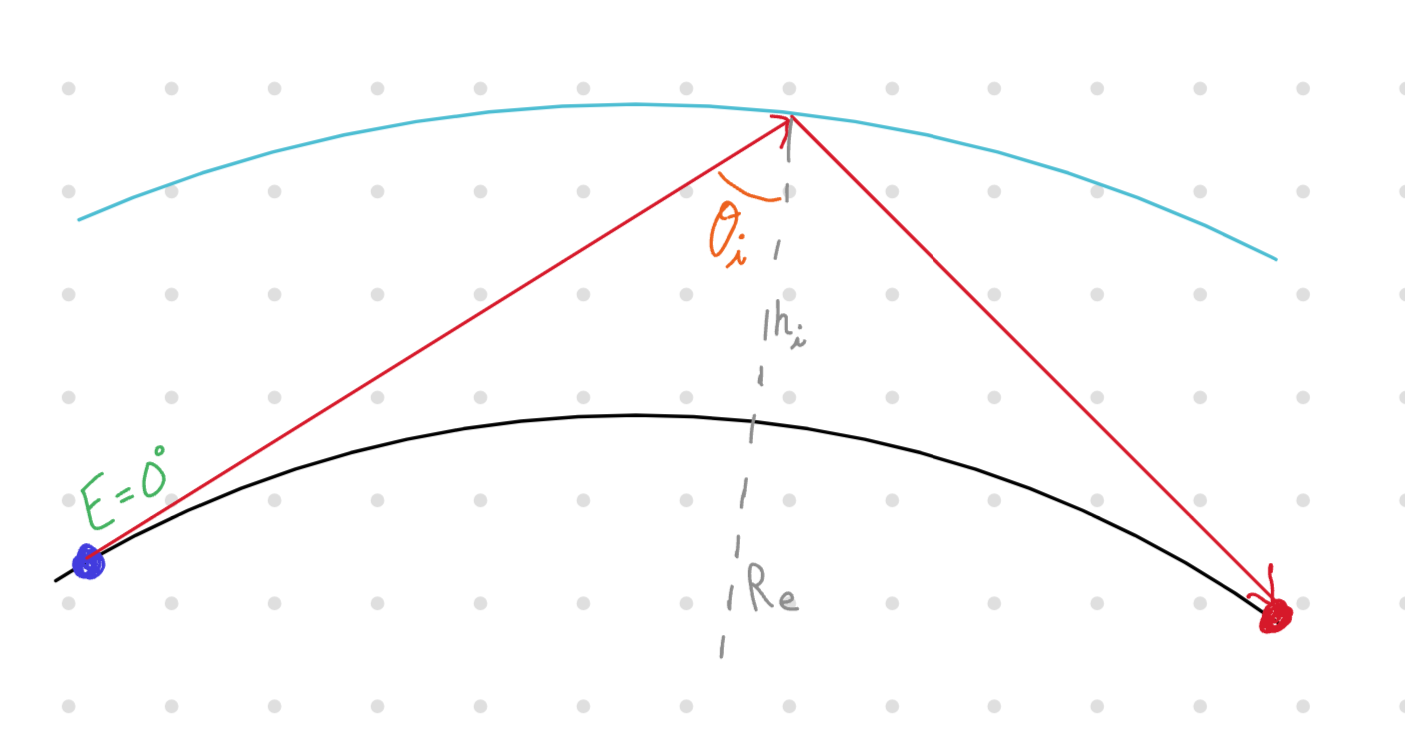
\includegraphics[width=1\linewidth]{grazing_angle.png}
            \end{figure}
            Grazing elevation $E=0^\circ \implies$ bigger $\theta_i$\\
            $\implies$ We can use higher frequencies and still not go over the critical angle ($\theta_i>\theta_c)$.\\
            \textbf{Reach longer distances.}
        \end{column}
        \begin{column}{0.48\textwidth}
            \begin{figure}
                \centering
                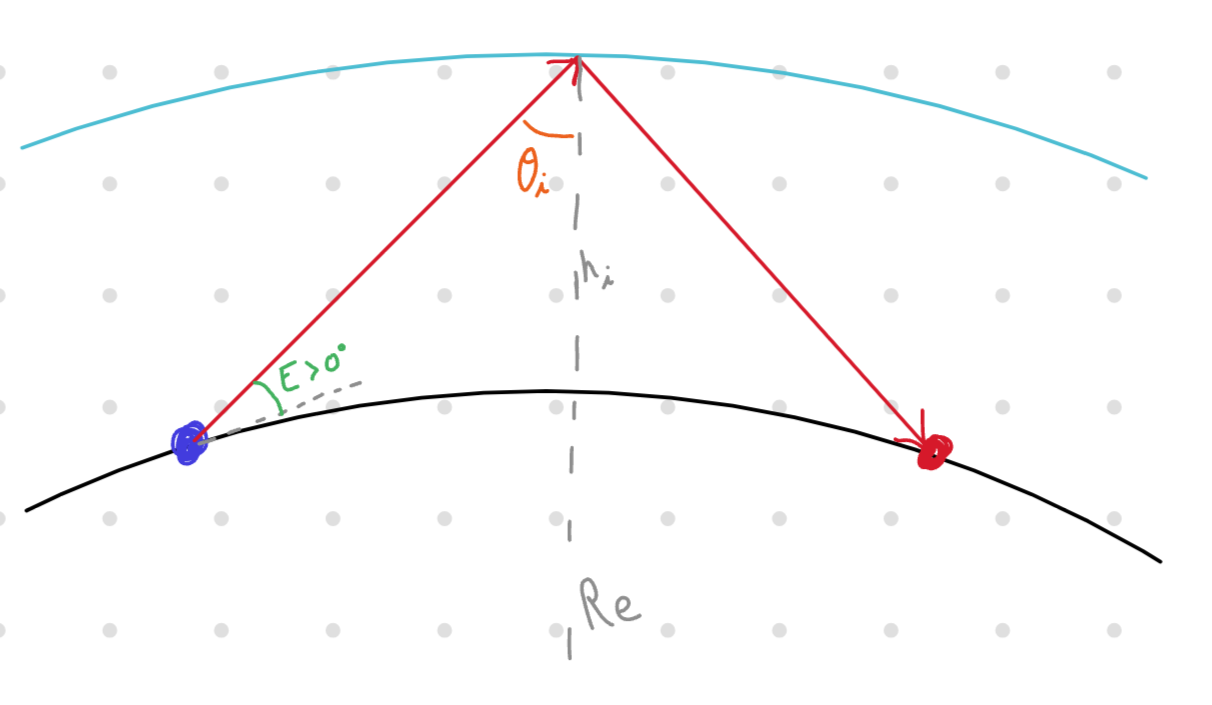
\includegraphics[width=1\linewidth]{higher-elevation-angle.png}
            \end{figure}
            Higher elevation E $\implies$ smaller $\theta_i$\\
            $\implies$ We have to use lower frequencies and to not go over the critical angle ($\theta_i>\theta_c)$.\\
            \textbf{Reach closer distances.}
        \end{column}
    \end{columns}
\end{frame}

\end{document}